\documentclass[10pt,twocolumn,letterpaper]{article}

% --- Page Geometry matching ICML / Top-Tier ML & Systems Conferences ---
\usepackage[
  letterpaper,
  top=1.0in,
  bottom=1.0in,
  left=0.875in,
  right=0.875in,
  columnsep=0.25in
]{geometry}

% --- Typography: Times Roman + Microtypography ---
\usepackage{times}
\usepackage{mathptmx}
\usepackage{microtype}
\usepackage[utf8]{inputenc}
\usepackage[T1]{fontenc}

% --- Mathematics & Theorems ---
\usepackage{amsmath,amsfonts,amssymb,amsthm}
\newtheorem{theorem}{Theorem}
\newtheorem{lemma}[theorem]{Lemma}
\newtheorem{definition}[theorem]{Definition}
\newtheorem{corollary}[theorem]{Corollary}

% --- Professional Graphics & Tables ---
\usepackage{graphicx}
\usepackage{booktabs}
\usepackage{array}
\usepackage{url}
\usepackage{cite}
\usepackage{textcomp}
\usepackage{tikz}
\usetikzlibrary{arrows,arrows.meta,positioning,shapes.geometric,calc,fit}

% --- Running Headers & Footers (ICML style) ---
\usepackage{fancyhdr}
\pagestyle{fancy}
\fancyhf{}
\fancyhead[C]{\small\itshape Architectural Foundations of Relational Joins and Multi-Table Query Optimization: Cross Products, Equi-Joins, Execution Algorithms, and Indexing Strategies in SQL Systems}
\fancyfoot[C]{\small\thepage}
\renewcommand{\headrulewidth}{0.4pt}
\renewcommand{\footrulewidth}{0pt}

% Suppress header on first page
\fancypagestyle{firstpage}{
  \fancyhf{}
  \fancyfoot[L]{\footnotesize\itshape Proceedings of Industrial \& Systems Database Architecture, 2026.}
  \fancyfoot[C]{\small\thepage}
  \renewcommand{\headrulewidth}{0pt}
}

% --- Compact Section Titles (ICML style: 1. Introduction, 1.1. Subheading) ---
\usepackage{titlesec}
\titleformat{\section}{\large\bfseries}{\thesection.}{0.5em}{}
\titleformat{\subsection}{\normalsize\bfseries}{\thesubsection.}{0.5em}{}
\titleformat{\subsubsection}{\small\bfseries}{\thesubsubsection.}{0.5em}{}
\titlespacing*{\section}{0pt}{1.5ex plus 0.5ex minus 0.2ex}{1.0ex plus 0.2ex}
\titlespacing*{\subsection}{0pt}{1.2ex plus 0.4ex minus 0.2ex}{0.8ex plus 0.2ex}
\titlespacing*{\subsubsection}{0pt}{1.0ex plus 0.3ex minus 0.2ex}{0.6ex plus 0.2ex}

% --- Listings Formatting for SQL & Code ---
\usepackage{listings}
\usepackage{xcolor}

\definecolor{codeblue}{rgb}{0.0,0.2,0.7}
\definecolor{codegreen}{rgb}{0,0.5,0}
\definecolor{codegray}{rgb}{0.4,0.4,0.4}
\definecolor{codepurple}{rgb}{0.5,0,0.7}
\definecolor{backcolour}{rgb}{0.98,0.98,0.98}

\lstdefinestyle{sqlStyle}{
    backgroundcolor=\color{backcolour},   
    commentstyle=\color{codegreen}\itshape,
    keywordstyle=\color{codeblue}\bfseries,
    numberstyle=\tiny\color{codegray},
    stringstyle=\color{codepurple},
    basicstyle=\ttfamily\scriptsize,
    breakatwhitespace=false,         
    breaklines=true,                 
    captionpos=b,                    
    keepspaces=true,                 
    numbers=none,
    showspaces=false,                
    showstringspaces=false,
    showtabs=false,                  
    tabsize=2,
    frame=single,
    rulecolor=\color{black!20}
}
\lstset{style=sqlStyle}

\begin{document}

\twocolumn[
  \begin{@twocolumnfalse}
    \begin{center}
      {\LARGE\bfseries {{TITLE}} \par}
      \vspace{1.0em}
      {\large\bfseries Pavan Gopala \par}
      \vspace{0.3em}
      {\small Database Systems and Relational Architecture Group \par}
      {\small\texttt{pavan@enterprise-sql.org} \par}
      \vspace{1.5em}
    \end{center}
  \end{@twocolumnfalse}
]

\thispagestyle{firstpage}

\begin{center}
  {\bfseries\large Abstract}
\end{center}
\vspace{-0.5em}
{\small In enterprise software architectures, relational database management systems (RDBMS) depend on multi-table joins and data query language (DQL) optimization to reconstruct normalized entity relationships with sub-millisecond latency. This paper presents an exhaustive systems engineering investigation of relational query execution, Cartesian cross products, equi-joins, asymmetric outer joins, and associative entity traversals derived from industrial database engines such as MySQL InnoDB and the canonical Sakila schema. We formalize the Boolean Precedence Hierarchy (the BODMAS of SQL) and dissect ANSI SQL Three-Valued Logic (3VL), tracing the epistemic semantics of NULL and the catastrophic failure modes of NOT IN subqueries and non-SARGable type coercions. We evaluate the performance collapse of deep LIMIT/OFFSET pagination, contrasting it against indexed Keyset cursors. We dissect the critical semantic boundary between join ON predicates and post-join WHERE filters, proving how improper predicate placement silently collapses Left Outer Joins into Inner Joins. We conduct a rigorous comparative analysis of physical join execution algorithms---Simple Nested Loop, Block Nested Loop (BNL), Index Nested Loop (INLJ), Hash Join, and Sort-Merge Join---tracing memory buffer dynamics and disk page I/O. Furthermore, we examine the Cost-Based Optimizer's (CBO) join ordering search space, driving table selection heuristics, and composite covering B+ Tree index design. Finally, we establish production safeguards against unconstrained table mutations via the \texttt{sql\_safe\_updates} directive. All discussions are accompanied by vector TikZ architectural diagrams, exact truth matrices, and production-grade SQL code listings.}

\vspace{1.0em}
\noindent\textbf{Keywords:} Relational Databases, SQL Joins, Query Optimization, Predicate Pushdown, Three-Valued Logic, Hash Join, Index Nested Loop, InnoDB Storage Engine.
\vspace{1.2em}

\section{Introduction}
\label{sec:intro}

Modern enterprise computing infrastructures depend fundamentally on Relational Database Management Systems (RDBMS) such as MySQL (InnoDB), PostgreSQL, and Oracle to process high-concurrency transactional queries with ACID guarantees and deterministic consistency. At the foundation of the relational model, formalized by Edgar F.~Codd in 1970 \cite{codd1970}, is the principle of relational normalization. Normalization decomposes application entities across multiple discrete relations to eliminate structural anomalies:
\begin{enumerate}
    \item \textbf{Update Anomalies}: Preventing inconsistent partial state transitions when a shared entity attribute is modified in one record but remains unchanged in another.
    \item \textbf{Insertion Anomalies}: Enabling independent recording of entity metadata prior to the existence of associated operational records (e.g., establishing a catalog language before films are produced in that language).
    \item \textbf{Deletion Anomalies}: Preventing the accidental purging of fundamental business entities when associated transactional records are deleted.
\end{enumerate}

\begin{figure*}[htbp]
\centering
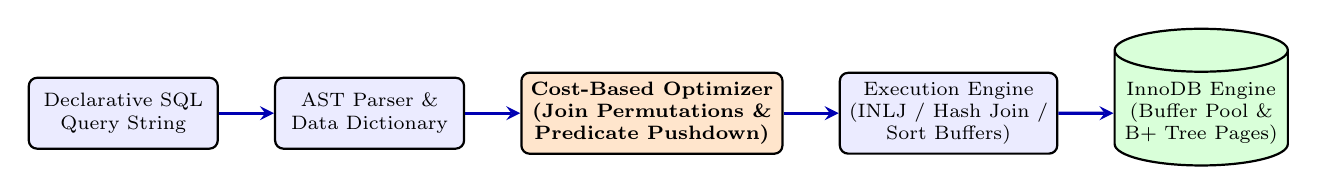
\begin{tikzpicture}[
    node distance=0.8cm and 0.9cm,
    box/.style={draw, rectangle, rounded corners=3pt, thick, align=center, fill=blue!8, minimum width=2.4cm, minimum height=0.9cm, font=\scriptsize},
    hlbox/.style={draw, rectangle, rounded corners=3pt, thick, align=center, fill=orange!20, minimum width=2.6cm, minimum height=0.9cm, font=\scriptsize\bfseries},
    storage/.style={draw, cylinder, shape border rotate=90, aspect=0.25, thick, align=center, fill=green!15, minimum width=2.2cm, minimum height=1.1cm, font=\scriptsize},
    arr/.style={->, >=stealth, very thick, color=blue!70!black}
]
    \node[box] (sql) {Declarative SQL\\Query String};
    \node[box, right=0.7cm of sql] (parser) {AST Parser \&\\Data Dictionary};
    \node[hlbox, right=0.7cm of parser] (cbo) {Cost-Based Optimizer\\(Join Permutations \&\\Predicate Pushdown)};
    \node[box, right=0.7cm of cbo] (exec) {Execution Engine\\(INLJ / Hash Join /\\Sort Buffers)};
    \node[storage, right=0.7cm of exec] (innodb) {InnoDB Engine\\(Buffer Pool \&\\B+ Tree Pages)};
    
    \draw[arr] (sql) -- (parser);
    \draw[arr] (parser) -- (cbo);
    \draw[arr] (cbo) -- (exec);
    \draw[arr] (exec) -- (innodb);
\end{tikzpicture}
\caption{The Relational Multi-Table Query Processing Pipeline. The Cost-Based Optimizer (CBO) evaluates table statistics, index selectivity, and join graph permutations to construct an optimal execution plan, pushing filters down before streaming records through join algorithms.}
\label{fig:pipeline}
\end{figure*}

However, while normalization decomposes data for storage integrity, business workflows demand composite representations. An entertainment catalog cannot display isolated numeric keys; it must present film titles alongside spoken languages, director biographies, and actor filmographies. To reconstruct these composite relationships on demand, relational engines execute \textbf{Relational Joins}.

Unlike imperative application-level joins---where an application queries a parent table, iterates over rows in application memory, and fires secondary queries in an imperative loop (the catastrophic $N+1$ query problem)---SQL joins are declarative. The application specifies the target relational schema and matching predicates, delegating physical execution to the database query planner. The database engine executes multi-table joins within the server's buffer pool, leveraging clustered B+ Tree index traversals, in-memory hash tables, and vector pipelining with sub-millisecond latency.

Based on production query traces and foundational database engineering principles using the canonical Sakila schema \cite{sakila2024}, this research paper presents an exhaustive architectural analysis of Data Query Language (DQL) predicate evaluation, Boolean precedence hierarchies, three-valued logic, and multi-table join mechanics. Following the empirical and mathematical rigor of classical systems literature, we formalize relational join calculus, derive algorithmic execution complexities, and trace physical memory buffer behaviors.

% -----------------------------------------------------------------------------
\section{Single-Relation Selection and Projection Foundations}
\label{sec:projection}

Before analyzing cross-relation join operators, we establish the fundamental mechanics of the projection ($\pi$) and selection ($\sigma$) operators within single-table execution.

\subsection{Scalar Evaluations and Constant Expressions}
In SQL, the \texttt{SELECT} clause is not restricted to projecting stored table attributes; it serves as a general expression evaluation engine:
\begin{lstlisting}[language=SQL]
-- 1. Literal integer evaluation (print equivalent):
SELECT 55 AS num;

-- 2. Non-deterministic temporal system evaluation:
SELECT NOW() AS curr_ts;

-- 3. Boolean primitive evaluation (returns 1 for TRUE):
SELECT 3 = 3 AS res;

-- 4. Deterministic mathematical function invocation:
SELECT ROUND(12.356, 2) AS num; -- Returns 12.36
\end{lstlisting}

When scalar expressions are evaluated against a relation (e.g., \texttt{SELECT title FROM film;}), the execution engine evaluates the projection expression once for every qualifying tuple emitted by upstream filtering stages.

\subsection{Tuple-Level Distinctness via the DISTINCT Operator}
A frequent architectural misunderstanding in relational database design concerns the operational scope of the \texttt{DISTINCT} modifier. The \texttt{DISTINCT} keyword does not apply to an individual column; it enforces uniqueness across the \textbf{entire projected attribute set} (tuple):

\begin{lstlisting}[language=SQL]
-- Single-attribute distinctness:
SELECT DISTINCT rating FROM film;
-- Multi-attribute tuple distinctness:
SELECT DISTINCT rental_rate, rental_duration FROM film;
\end{lstlisting}

\begin{definition}[Tuple Projection Distinctness]
Given a relation $R$ with schema $\mathcal{R}$ and attribute subset $A \subseteq \mathcal{R}$, the distinct projection $\pi^*_{A}(R)$ is the set of unique tuples:
\begin{equation}
\pi^*_{A}(R) = \{ t[A] \mid t \in R \}
\end{equation}
Duplicate suppression occurs if and only if two tuples $t_1, t_2 \in R$ satisfy $t_1[A] = t_2[A]$ identically across all attributes in $A$.
\end{definition}

If two rows share an identical \texttt{rental\_rate} of 4.99 but possess different \texttt{rental\_duration} values (e.g., 3 days versus 5 days), both tuples are retained in the output set.

\subsection{Physical Execution Mechanics of DISTINCT}
The query execution engine implements distinctness through two primary physical strategies:
\begin{enumerate}
    \item \textbf{B+ Tree Index Stream Aggregation}: When a composite secondary index exists on the projected columns in matching order, the engine traverses the index sequentially. Because the B+ Tree leaf pages are physically sorted, duplicate tuples are stored contiguously. The engine performs a streaming linear scan, emitting the first tuple of each run and skipping adjacent duplicates in $\mathcal{O}(N)$ time with zero auxiliary memory allocation.
    \item \textbf{Temporary Hash Table or Filesort}: In the absence of an index, the engine allocates an in-memory hash table in thread memory (bounded by \texttt{tmp\_table\_size}). Incoming rows are hashed on the projected composite key. If the unique tuple set exceeds available memory, the intermediate result spills to disk, triggering a multi-pass merge filesort that dramatically inflates disk I/O.
\end{enumerate}

% -----------------------------------------------------------------------------
\section{Predicate Evaluation Architecture and Boolean Precedence}
\label{sec:filtering}

The \texttt{WHERE} clause enforces relational selection ($\sigma$), filtering candidate rows from the physical storage scan.

\subsection{Case Sensitivity, Collation, and The BINARY Operator}
By default, modern MySQL installations operate under case-insensitive collations (such as \texttt{utf8mb4\_0900\_ai\_ci}):
\begin{lstlisting}[language=SQL]
SELECT title, rating FROM film WHERE rating = 'PG-13';
\end{lstlisting}
Under case-insensitive collation, string comparisons ignore character casing: \texttt{'PG-13'} matches \texttt{'pg-13'} and \texttt{'Pg-13'}. When byte-exact lexicographical matching is required, the \texttt{BINARY} cast forces byte-level evaluation:
\begin{lstlisting}[language=SQL]
SELECT title, rating FROM film
WHERE BINARY rating = 'PG-13' OR BINARY rating = 'G';
\end{lstlisting}
The \texttt{BINARY} operator treats characters as raw byte sequences, enforcing exact ASCII/UTF-8 byte identity. Relational inequality is expressed symmetrically via \texttt{!=} or the ANSI-standard \texttt{<>}:
\begin{lstlisting}[language=SQL]
SELECT title, rating FROM film WHERE rating != 'PG-13';
SELECT title, rating FROM film WHERE rating <> 'PG-13';
\end{lstlisting}

\subsection{The Boolean Precedence Hierarchy (The BODMAS of SQL)}
Just as standard arithmetic enforces operator precedence where multiplication precedes addition, relational database query engines enforce a strict Boolean Precedence Hierarchy:
\begin{center}
\textbf{The \texttt{AND} operator evaluates with strictly higher precedence than the \texttt{OR} operator.}
\end{center}

Consider the following unparenthesized compound filter:
\begin{lstlisting}[language=SQL]
-- Ambiguous compound boolean condition:
SELECT * FROM film 
WHERE rating = 'PG-13' OR rental_rate = 0.99 AND release_year = 2006;
\end{lstlisting}

Because \texttt{AND} binds tighter than \texttt{OR}, the query parser constructs the following Abstract Syntax Tree:
\begin{lstlisting}[language=SQL]
-- Internal evaluation tree executed by the engine:
SELECT * FROM film 
WHERE rating = 'PG-13' OR (rental_rate = 0.99 AND release_year = 2006);
\end{lstlisting}

This produces catastrophic logical bugs in enterprise systems:
\begin{itemize}
    \item The query returns \textbf{every single film} with rating \texttt{'PG-13'} regardless of its release year.
    \item If the business requirement intended to restrict all results strictly to the year 2006, the unparenthesized query silently violates business rules.
\end{itemize}

\subsubsection{Defensive Engineering Guideline}
Software engineers must \textbf{always enforce explicit parentheses} around disjunctive groups:
\begin{lstlisting}[language=SQL]
-- Correct, unambiguous business logic:
SELECT * FROM film 
WHERE (rating = 'PG-13' OR rental_rate = 0.99) 
  AND release_year = 2006;
\end{lstlisting}

Table~\ref{tab:precedence} details the operational precedence hierarchy in relational engines.

\begin{table}[htbp]
\caption{SQL Operator Precedence Hierarchy (Highest to Lowest)}
\label{tab:precedence}
\centering
\scriptsize
\begin{tabular}{lll}
\toprule
\textbf{Rank} & \textbf{Operator Class} & \textbf{SQL Operators} \\
\midrule
1 (Highest) & Grouping \& Scope & Parentheses \texttt{()} \\
2 & Member Access & JSON extraction \texttt{->}, \texttt{->>} \\
3 & Unary Operators & Unary minus \texttt{-}, Bitwise inversion \texttt{\~{}} \\
4 & Multiplicative & Multiplication \texttt{*}, Division \texttt{/}, Modulo \texttt{\%} \\
5 & Additive & Addition \texttt{+}, Subtraction \texttt{-} \\
6 & Relational Comparisons & \texttt{=}, \texttt{!=}, \texttt{<>}, \texttt{<}, \texttt{<=}, \texttt{>}, \texttt{>=}, \texttt{LIKE}, \texttt{IN} \\
7 & Logical Negation & \texttt{NOT} \\
\textbf{8} & \textbf{Logical Conjunction} & \textbf{\texttt{AND}} \\
\textbf{9 (Lowest)} & \textbf{Logical Disjunction} & \textbf{\texttt{OR}} \\
\bottomrule
\end{tabular}
\end{table}

\subsection{Set Membership and Range Predicates}
When evaluating an attribute against discrete values, the \texttt{IN} operator provides syntactic conciseness and query engine optimization compared to chained \texttt{OR} expressions:
\begin{lstlisting}[language=SQL]
-- Chained OR representation:
SELECT title, rental_duration FROM film
WHERE rental_duration = 3 OR rental_duration = 4 OR rental_duration = 6;

-- Equivalent IN set membership representation:
SELECT title, rental_duration FROM film
WHERE rental_duration IN (3, 4, 6);
\end{lstlisting}
Internally, the query planner sorts the constant set into an array and performs binary search point lookups. Conversely, \texttt{NOT IN} translates via De Morgan's laws into chained inequalities joined by \texttt{AND}:
\begin{lstlisting}[language=SQL]
SELECT title, rental_duration FROM film 
WHERE rental_duration NOT IN (3, 4, 6);
-- De Morgan equivalence:
SELECT title, rental_duration FROM film 
WHERE rental_duration <> 3 AND rental_duration <> 4 AND rental_duration <> 6;
\end{lstlisting}

\subsection{Range and Substring Search Mechanics}
The \texttt{BETWEEN} operator enforces a closed interval inclusive of both boundaries:
\begin{lstlisting}[language=SQL]
SELECT rental_duration FROM film WHERE rental_duration BETWEEN 1 AND 6;
-- Exact boundary equivalence:
-- rental_duration >= 1 AND rental_duration <= 6
\end{lstlisting}

In pattern matching via \texttt{LIKE}, wildcards dictate B+ Tree index utilization (Search Argument Able / SARGability):
\begin{itemize}
    \item \textbf{Leading Wildcards (\texttt{'\%love\%'})}: The engine cannot determine the starting character of the string. B+ Tree index seeks are disabled, forcing an exhaustive full table scan across all leaf blocks.
    \item \textbf{Trailing Wildcards (\texttt{'love\%'})}: The engine executes an index range scan on the B+ Tree, seeking directly to the first key with prefix \texttt{'love'} and scanning leaf nodes until the prefix boundary is reached.
\end{itemize}

% -----------------------------------------------------------------------------
\section{Three-Valued Logic (3VL) and Epistemic NULL Semantics}
\label{sec:three_valued_logic}

The handling of \texttt{NULL} values represents one of the most prolific sources of logic bugs in relational database systems.

\subsection{The Epistemic Nature of NULL}
In relational database systems, \texttt{NULL} does \textbf{not} represent zero ($0$), nor does it represent an empty string (\texttt{""}). \texttt{NULL} signifies an \textbf{epistemic state of unknown, missing, or unassigned data}.

Because \texttt{NULL} represents an unknown quantity, it breaks classical two-valued Boolean logic. In classical logic, every proposition $P$ is either True or False ($P \lor \neg P = \text{TRUE}$). In SQL, proposition evaluation is governed by Three-Valued Logic (3VL) over the truth space:
\begin{equation}
\mathbb{T}_{\text{SQL}} = \{ \text{TRUE}, \text{FALSE}, \text{UNKNOWN} \}
\end{equation}

\subsection{Identity Comparison Failures}
Because \texttt{NULL} denotes missing information, identity comparisons yield \texttt{UNKNOWN}:
\begin{lstlisting}[language=SQL]
SELECT 3 = NULL;     -- Evaluates to NULL (UNKNOWN), NOT False!
SELECT NULL = NULL;  -- Evaluates to NULL (UNKNOWN), NOT True!
\end{lstlisting}
The engine reasons: ``Is an unknown quantity equal to 3? The answer is unknown.'' Similarly: ``Are two independently unknown quantities identical? The answer is unknown.''

\begin{figure*}[htbp]
\centering
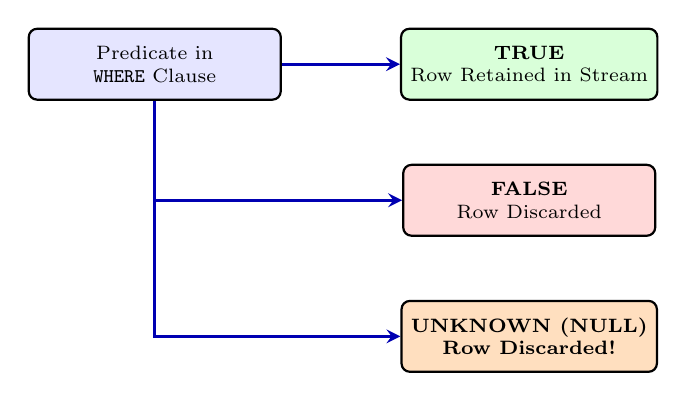
\begin{tikzpicture}[
    box/.style={draw, rectangle, rounded corners=3pt, thick, align=center, fill=blue!10, minimum width=3.2cm, minimum height=0.9cm, font=\scriptsize},
    hlbox/.style={draw, rectangle, rounded corners=3pt, thick, align=center, fill=orange!25, minimum width=3.2cm, minimum height=0.9cm, font=\scriptsize\bfseries},
    resbox/.style={draw, rectangle, rounded corners=3pt, thick, align=center, fill=green!15, minimum width=3.2cm, minimum height=0.9cm, font=\scriptsize},
    dropbox/.style={draw, rectangle, rounded corners=3pt, thick, align=center, fill=red!15, minimum width=3.2cm, minimum height=0.9cm, font=\scriptsize},
    arr/.style={->, >=stealth, very thick, color=blue!70!black}
]
    \node[box] (expr) {Predicate in\\ \texttt{WHERE} Clause};
    \node[resbox, right=1.5cm of expr] (true) {\textbf{TRUE}\\Row Retained in Stream};
    \node[dropbox, below=0.8cm of true] (false) {\textbf{FALSE}\\Row Discarded};
    \node[hlbox, below=0.8cm of false] (unk) {\textbf{UNKNOWN (NULL)}\\Row Discarded!};
    
    \draw[arr] (expr) -- (true);
    \draw[arr] (expr) |- (false);
    \draw[arr] (expr) |- (unk);
\end{tikzpicture}
\caption{Three-Valued Logic in Relational Filtering. Candidate tuples are retained in the result stream if and only if the \texttt{WHERE} condition evaluates strictly to \texttt{TRUE}. Expressions evaluating to \texttt{UNKNOWN} are discarded alongside \texttt{FALSE}.}
\label{fig:3vl}
\end{figure*}

\subsection{Truth Matrices and The Fatal NOT IN Null Trap}
Table~\ref{tab:3vl_truth} formalizes the complete operational behavior of SQL boolean operators when interacting with unknown states.

\begin{table}[htbp]
\caption{ANSI SQL Three-Valued Logic (3VL) Truth Matrix}
\label{tab:3vl_truth}
\centering
\scriptsize
\begin{tabular}{ccccc}
\toprule
\textbf{Operand A} & \textbf{Operand B} & \textbf{A AND B} & \textbf{A OR B} & \textbf{NOT A} \\
\midrule
TRUE & TRUE & TRUE & TRUE & FALSE \\
TRUE & FALSE & FALSE & TRUE & FALSE \\
TRUE & UNKNOWN & \textbf{UNKNOWN} & \textbf{TRUE} & FALSE \\
\midrule
FALSE & FALSE & FALSE & FALSE & TRUE \\
FALSE & UNKNOWN & \textbf{FALSE} & \textbf{UNKNOWN} & TRUE \\
\midrule
UNKNOWN & UNKNOWN & \textbf{UNKNOWN} & \textbf{UNKNOWN} & \textbf{UNKNOWN} \\
\bottomrule
\end{tabular}
\end{table}

To check for null states in classical two-valued logic, SQL provides the dedicated unary predicates \texttt{IS NULL} and \texttt{IS NOT NULL}:
\begin{lstlisting}[language=SQL]
SELECT 3 IS NULL;        -- FALSE
SELECT 3 IS NOT NULL;    -- TRUE
SELECT NULL IS NULL;     -- TRUE
SELECT NULL IS NOT NULL; -- FALSE
\end{lstlisting}

\subsubsection{The Fatal NOT IN Null Trap}
A notorious production failure occurs when evaluating a \texttt{NOT IN} predicate against a subquery or list containing a \texttt{NULL}:
\begin{lstlisting}[language=SQL]
-- Target candidate set contains a NULL:
SELECT * FROM film WHERE rental_duration NOT IN (3, 4, NULL);
\end{lstlisting}
Under De Morgan's expansion, this statement evaluates to:
\begin{equation}
(\text{dur} \neq 3) \land (\text{dur} \neq 4) \land (\text{dur} \neq \text{NULL})
\end{equation}
Because $(\text{dur} \neq \text{NULL})$ evaluates to \textbf{\texttt{UNKNOWN}}, the entire compound conjunction evaluates to \textbf{\texttt{UNKNOWN}} for every single row in the database. The query returns \textbf{zero rows}, silently dropping all records! Production systems must use \texttt{NOT EXISTS} or explicitly filter nulls from candidate sets.

\subsection{Implicit Type Coercion and Index SARGability}
When expressions of differing types are compared, MySQL executes implicit type coercion:
\begin{lstlisting}[language=SQL]
SELECT 3 = '3';                -- String coerced to numeric -> TRUE
SELECT 12890092 = '12890092';  -- TRUE
SELECT binary 'a' = 'A';       -- Binary comparison -> FALSE
\end{lstlisting}

When a query compares an indexed string column against a numeric literal:
\begin{lstlisting}[language=SQL]
-- Indexed column: phone_number VARCHAR(20)
SELECT * FROM customer WHERE phone_number = 9876543210;
\end{lstlisting}
Under MySQL type coercion rules, comparing a string column with an integer causes the engine to cast the \textbf{column to double}, rewriting the predicate internally as:
\begin{lstlisting}[language=SQL]
SELECT * FROM customer WHERE CAST(phone_number AS DOUBLE) = 9876543210;
\end{lstlisting}
Wrapping an indexed column in a function destroys B+ Tree traversal, forcing an exhaustive full table scan across millions of disk pages. Passing literals matching the column's data type (\texttt{'9876543210'}) restores instant sub-millisecond B+ Tree index seeks.

% -----------------------------------------------------------------------------
\section{Physical Execution Ordering and Pagination Dynamics}
\label{sec:sort_pushdown}

A foundational optimization in relational systems is determining the sequence of physical execution steps when a query specifies both a filtering predicate (\texttt{WHERE}) and a sorting directive (\texttt{ORDER BY}):

\begin{lstlisting}[language=SQL]
SELECT * FROM film 
WHERE rating = 'PG-13' 
ORDER BY title DESC;
\end{lstlisting}

\subsection{Algorithmic Analysis of Execution Options}
Let $N$ denote the total number of rows in the table, and $X$ denote the number of rows satisfying \texttt{rating = 'PG-13'} (where $X \ll N$):
\begin{itemize}
    \item \textbf{Option A (Sort-First, Filter-Second)}: The engine loads all $N$ rows into a memory sort buffer, executes a full sort in $\mathcal{O}(N \log_2 N)$ comparisons, and subsequently filters the sorted stream, incurring a total operational cost of:
    \begin{equation}
    C_{\text{sort-first}} = \mathcal{O}(N \log_2 N + N)
    \end{equation}
    \item \textbf{Option B (Filter-First, Sort-Second / Predicate Pushdown)}: The engine scans the table (or uses an index on \texttt{rating}), discards non-matching rows immediately, and loads only the surviving $X$ rows into the filesort buffer. The sort executes in $\mathcal{O}(X \log_2 X)$ comparisons, incurring a total operational cost of:
    \begin{equation}
    C_{\text{pushdown}} = \mathcal{O}(N + X \log_2 X)
    \end{equation}
\end{itemize}

Because $X \ll N$ in selective queries, Option B dramatically reduces CPU cache thrashing and memory consumption. All production relational optimizers enforce Predicate Pushdown as a core execution invariant.

\begin{figure}[htbp]
\centering
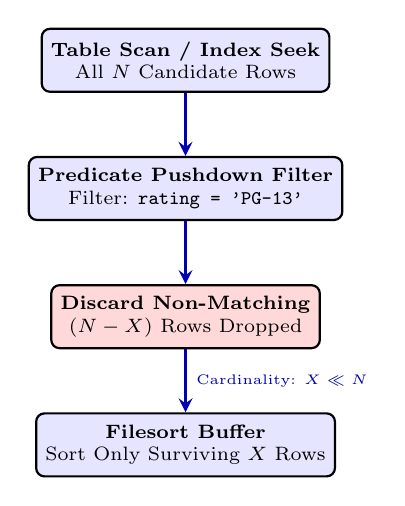
\begin{tikzpicture}[
    box/.style={draw, rectangle, rounded corners=3pt, thick, align=center, fill=blue!10, minimum width=3.0cm, minimum height=0.8cm, font=\scriptsize},
    discard/.style={draw, rectangle, rounded corners=3pt, thick, align=center, fill=red!15, minimum width=3.0cm, minimum height=0.8cm, font=\scriptsize},
    arr/.style={->, >=stealth, very thick, color=blue!70!black}
]
    \node[box] (scan) {\textbf{Table Scan / Index Seek}\\All $N$ Candidate Rows};
    \node[box, below=0.8cm of scan] (filter) {\textbf{Predicate Pushdown Filter}\\Filter: \texttt{rating = 'PG-13'}};
    \node[discard, below=0.8cm of filter] (drop) {\textbf{Discard Non-Matching}\\$(N - X)$ Rows Dropped};
    \node[box, below=0.8cm of drop] (sort) {\textbf{Filesort Buffer}\\Sort Only Surviving $X$ Rows};
    
    \draw[arr] (scan) -- (filter);
    \draw[arr] (filter) -- (drop);
    \draw[arr] (drop) -- node[right, font=\tiny] {Cardinality: $X \ll N$} (sort);
\end{tikzpicture}
\caption{Predicate Pushdown Mechanics. Filtering rows prior to sort buffer allocation minimizes memory consumption and prevents temporary disk spills.}
\label{fig:pushdown}
\end{figure}

\subsection{Multi-Column Hierarchical Sorting and Deterministic Tie-Breakers}
When sorting by multiple attributes:
\begin{lstlisting}[language=SQL]
SELECT student_id, psp, age, name 
FROM students 
ORDER BY psp DESC, age ASC, student_id ASC;
\end{lstlisting}
The engine evaluates keys hierarchically:
\begin{enumerate}
    \item \textbf{Primary Sort Key (\texttt{psp DESC})}: Rows are ordered by problem solving percentage in descending order.
    \item \textbf{Secondary Key (\texttt{age ASC})}: If two students share an identical \texttt{psp}, the tie is resolved by ordering by age ascending.
    \item \textbf{Deterministic Anchor (\texttt{student\_id ASC})}: If both \texttt{psp} and \texttt{age} tie, the Primary Key provides an unambiguous, deterministic ordering.
\end{enumerate}

\subsubsection{The Indeterminate Ordering Anomaly}
In relational theory, a relation is an unordered set of tuples. If an \texttt{ORDER BY} clause fails to resolve ties down to a unique key, the engine emits tied rows in arbitrary physical storage order. Across database read replicas or successive pagination queries, tied rows switch positions randomly. Systems engineers must \textbf{always append the Primary Key} to sort specifications to guarantee deterministic results.

\subsection{Interaction Between DISTINCT and ORDER BY}
Standard ANSI SQL (SQL:1999) enforces a strict syntactic constraint:
\begin{center}
\textit{Any column appearing in the \texttt{ORDER BY} clause MUST be present in the \texttt{SELECT DISTINCT} projection list.}
\end{center}
Consider the invalid query:
\begin{lstlisting}[language=SQL]
-- Fails with MySQL Error 3065 in strict mode:
SELECT DISTINCT title, rental_duration FROM film ORDER BY rating;
\end{lstlisting}
If multiple rows share identical \texttt{title} and \texttt{rental\_duration} values but possess divergent \texttt{rating} values, the engine collates them into a single output tuple. If that collapsed tuple were sorted by \texttt{rating}, the engine faces an insoluble paradox: which rating determines its position? To eliminate non-determinism, SQL standards require sorted attributes to exist in the projected tuple.

\subsection{Pagination Architecture: LIMIT/OFFSET Degradation vs. Keyset Cursors}
Result set windowing is commonly implemented via \texttt{LIMIT} and \texttt{OFFSET}:
\begin{lstlisting}[language=SQL]
-- Retrieve page 2 (rows 11 through 30):
SELECT * FROM film 
WHERE film_id BETWEEN 10 AND 30 
ORDER BY film_id ASC 
LIMIT 20 OFFSET 10;
\end{lstlisting}

\subsubsection{The Offset Performance Cliff}
While \texttt{OFFSET} is intuitive for small page offsets, it collapses under deep pagination:
\begin{lstlisting}[language=SQL]
SELECT * FROM transactions ORDER BY id ASC LIMIT 20 OFFSET 10000000;
\end{lstlisting}
Because variable-length rows prevent jumping directly to row 10,000,000, the engine must physically read all 10,000,020 rows from disk or index buffers, only to discard the first 10,000,000 rows. Response latency degrades from milliseconds to tens of seconds.

\subsubsection{Keyset (Cursor-Based) Pagination}
Enterprise systems eliminate this degradation using Keyset (Cursor-Based) pagination:
\begin{lstlisting}[language=SQL]
-- High-performance Keyset Pagination:
SELECT * FROM transactions 
WHERE id > 10000000 
ORDER BY id ASC 
LIMIT 20;
\end{lstlisting}
By seeking on the indexed primary key \texttt{id}, the storage engine traverses the B+ Tree index in $\mathcal{O}(\log N)$ time, scanning exactly 20 physical records regardless of offset depth.

\subsubsection{The N-th Highest Salary Pattern}
Retrieving the second-highest salary while handling duplicate compensation tiers is formulated using \texttt{DISTINCT} and \texttt{OFFSET}:
\begin{lstlisting}[language=SQL]
SELECT DISTINCT salary 
FROM employees 
ORDER BY salary DESC 
LIMIT 1 OFFSET 1;
\end{lstlisting}
The \texttt{DISTINCT} modifier collapses tied top salaries into a single tier, enabling \texttt{OFFSET 1} to isolate the true second-highest compensation level.

% -----------------------------------------------------------------------------
\section{The Cartesian Cross Product ($R \times S$): Theoretical Basis and Hazards}
\label{sec:cartesian}

When multiple relations are joined without an explicit join predicate or \texttt{WHERE} clause, the database engine computes the \textbf{Cartesian Cross Product}.

\subsection{Theoretical Definition and Cardinality}
\begin{definition}[Cartesian Product]
Given two relations $R(A_1, \dots, A_n)$ and $S(B_1, \dots, B_m)$, the Cartesian product $R \times S$ produces a composite relation containing every possible concatenation of tuples:
\begin{equation}
R \times S = \{ (r_1, \dots, r_n, s_1, \dots, s_m) \mid r \in R \land s \in S \}
\end{equation}
The cardinality of the Cartesian product is strictly multiplicative:
\begin{equation}
|R \times S| = |R| \cdot |S|
\end{equation}
\end{definition}

\subsection{SQL Formulation and Production Traps}
In SQL, a Cartesian product is produced by listing relations separated by commas or using the \texttt{JOIN} / \texttt{CROSS JOIN} syntax without an \texttt{ON} predicate:
\begin{lstlisting}[language=SQL]
-- Cartesian product of film and language relations:
SELECT * FROM film JOIN language;
-- Equivalent comma-separated syntax:
SELECT * FROM film, language;
\end{lstlisting}

In the Sakila database, the \texttt{film} table contains 1,000 rows, and the \texttt{language} table contains 6 rows. The query evaluates to:
\begin{equation*}
1,000 \times 6 = 6,000 \text{ rows}
\end{equation*}

\begin{figure*}[htbp]
\centering
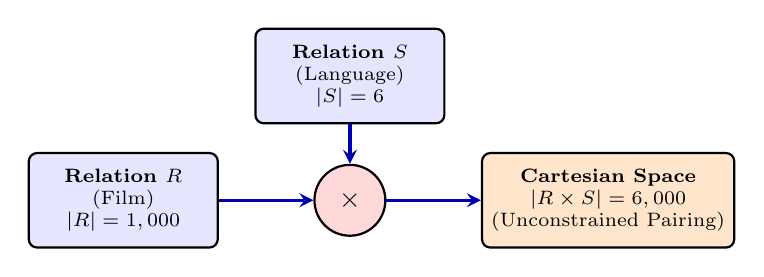
\begin{tikzpicture}[
    rel/.style={draw, rectangle, rounded corners=3pt, thick, align=center, fill=blue!10, minimum width=2.4cm, minimum height=1.2cm, font=\scriptsize},
    cross/.style={draw, circle, thick, align=center, fill=red!15, minimum size=0.9cm, font=\normalsize\bfseries},
    result/.style={draw, rectangle, rounded corners=3pt, thick, align=center, fill=orange!20, minimum width=3.0cm, minimum height=1.2cm, font=\scriptsize},
    arr/.style={->, >=stealth, very thick, color=blue!70!black}
]
    \node[rel] (r) {\textbf{Relation $R$}\\(Film)\\$|R| = 1,000$};
    \node[cross, right=1.2cm of r] (x) {$\times$};
    \node[rel, above=0.5cm of x] (s) {\textbf{Relation $S$}\\(Language)\\$|S| = 6$};
    \node[result, right=1.2cm of x] (res) {\textbf{Cartesian Space}\\$|R \times S| = 6,000$\\(Unconstrained Pairing)};
    
    \draw[arr] (r) -- (x);
    \draw[arr] (s) -- (x);
    \draw[arr] (x) -- (res);
\end{tikzpicture}
\caption{The Cartesian Cross Product. Every row of relation $R$ is paired unconditionally with every row of relation $S$, resulting in multiplicative tuple expansion.}
\label{fig:cartesian}
\end{figure*}

\subsubsection{Catastrophic Cartesian Explosions in Enterprise Systems}
While a 6,000-row Cartesian product is trivial, real-world relations exhibit massive tuple counts. Suppose an unconstrained join is executed between a customer relation ($|C| = 10^6$ rows) and an order relation ($|O| = 10^7$ rows):
\begin{equation*}
|C \times O| = 10^6 \times 10^7 = 10^{13} \text{ tuples (10 Trillion rows!)}
\end{equation*}
At 100 bytes per tuple, this intermediate result represents \textbf{1 Petabyte of data}. Attempting to compute this query saturates disk buffers, causes extreme CPU thread locking, exhausts the server buffer pool, and triggers OS kernel out-of-memory (OOM) killer terminations.

% -----------------------------------------------------------------------------
\section{Inner Join Semantics, Table Aliasing, and Referential Integrity}
\label{sec:inner_join}

The \textbf{Inner Join} is the primary relational mechanism for reconnecting normalized entities based on referential integrity.

\subsection{Relational Algebra Equi-Join Definition}
\begin{definition}[Theta Join and Equi-Join]
In relational algebra, an Inner Join (Theta Join $\bowtie_\theta$) is defined as a selection predicate applied over the Cartesian product:
\begin{equation}
R \bowtie_\theta S = \sigma_\theta(R \times S)
\end{equation}
When the join condition $\theta$ specifies strict equality across common attributes $R.k = S.k$ (an \textbf{Equi-Join}):
\begin{equation}
R \bowtie_{R.k = S.k} S = \{ (r, s) \mid r \in R \land s \in S \land r.k = s.k \}
\end{equation}
\end{definition}

\subsection{SQL Formulation and Namespace Disambiguation}
In the Sakila database, the \texttt{film} entity references the \texttt{language} entity through the foreign key \texttt{film.language\_id}. To retrieve each film title alongside its human-readable language name:
\begin{lstlisting}[language=SQL]
SELECT f.title, l.name AS lang_name
FROM film f
INNER JOIN language l ON f.language_id = l.language_id;
\end{lstlisting}

\subsubsection{Architectural Principles of Table Aliasing}
Table aliasing (\texttt{film f}, \texttt{language l}) provides three critical architectural advantages:
\begin{enumerate}
    \item \textbf{Namespace Resolution}: Eliminates column ambiguity errors when both tables share attribute names (such as \texttt{language\_id} and \texttt{last\_update}).
    \item \textbf{Query Succinctness and Readability}: Reduces verbose multi-table path prefixes across complex multi-line SQL statements.
    \item \textbf{Self-Join Disambiguation}: Allows a single physical relation to be joined with itself (e.g., employee-manager organizational hierarchies) by creating distinct logical instances.
\end{enumerate}

\subsection{Matching Semantics and Tuple Pruning}
An Inner Join retains a tuple if and only if the join predicate evaluates to \texttt{TRUE}:
\begin{itemize}
    \item If a film record possesses a \texttt{language\_id} that does not exist in the \texttt{language} table, that film is discarded from the result set.
    \item If a language record exists in \texttt{language} that is not referenced by any film (e.g., Mandarin), that language is discarded from the result set.
    \item If either join key attribute contains \texttt{NULL}, the comparison \texttt{f.language\_id = l.language\_id} evaluates to \texttt{UNKNOWN} under 3VL, and the tuple is strictly discarded.
\end{itemize}

% -----------------------------------------------------------------------------
\section{Asymmetric Outer Joins and the Semantic Boundary: ON vs. WHERE}
\label{sec:outer_joins}

When business requirements demand preserving records that lack matching referential counterparts, standard Inner Joins are inadequate. Relational systems provide \textbf{Outer Joins}.

\subsection{Outer Join Taxonomy}
\begin{itemize}
    \item \textbf{Left Outer Join ($R \mathbin{\bowtie_{\text{left}}} S$)}: Preserves all tuples from the left relation $R$. If a tuple $r \in R$ finds no matching tuple in $S$ satisfying the join condition, $r$ is concatenated with synthetic \texttt{NULL} values for all attributes of $S$.
    \item \textbf{Right Outer Join ($R \mathbin{\bowtie_{\text{right}}} S$)}: Preserves all tuples from the right relation $S$, padding missing left-relation attributes with \texttt{NULL}.
    \item \textbf{Full Outer Join ($R \mathbin{\bowtie_{\text{full}}} S$)}: Preserves all tuples from both relations, synthesizing \texttt{NULL}s on either side when a match is absent.
\end{itemize}

\begin{figure*}[htbp]
\centering
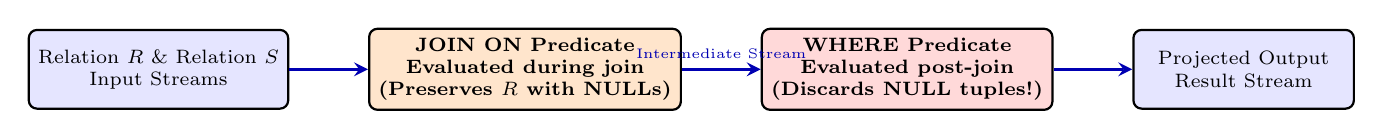
\begin{tikzpicture}[
    box/.style={draw, rectangle, rounded corners=3pt, thick, align=center, fill=blue!10, minimum width=2.8cm, minimum height=1.0cm, font=\scriptsize},
    onbox/.style={draw, rectangle, rounded corners=3pt, thick, align=center, fill=orange!20, minimum width=3.2cm, minimum height=1.0cm, font=\scriptsize\bfseries},
    wherebox/.style={draw, rectangle, rounded corners=3pt, thick, align=center, fill=red!15, minimum width=3.2cm, minimum height=1.0cm, font=\scriptsize\bfseries},
    arr/.style={->, >=stealth, very thick, color=blue!70!black}
]
    \node[box] (tables) {Relation $R$ \& Relation $S$\\Input Streams};
    \node[onbox, right=1.0cm of tables] (on) {\textbf{JOIN ON Predicate}\\Evaluated during join\\(Preserves $R$ with NULLs)};
    \node[wherebox, right=1.0cm of on] (where) {\textbf{WHERE Predicate}\\Evaluated post-join\\(Discards NULL tuples!)};
    \node[box, right=1.0cm of where] (out) {Projected Output\\Result Stream};
    
    \draw[arr] (tables) -- (on);
    \draw[arr] (on) -- node[above, font=\tiny] {Intermediate Stream} (where);
    \draw[arr] (where) -- (out);
\end{tikzpicture}
\caption{The Relational Execution Sequence for Joins. The \texttt{ON} predicate evaluates during tuple pairing (governing outer join preservation), while the \texttt{WHERE} predicate evaluates after intermediate tuple materialization.}
\label{fig:on_vs_where}
\end{figure*}

\subsection{The Semantic Boundary: ON vs. WHERE in Outer Joins}
One of the most insidious architectural bugs in relational SQL programming is misunderstanding the differing evaluation phases of the join predicate (\texttt{ON}) versus the post-join filter (\texttt{WHERE}).

\subsubsection{The Outer Join Collapse Anomaly}
Consider an application requirement: \textit{``Retrieve all films, and for films produced in English, show the language name.''}

Consider the incorrect implementation:
\begin{lstlisting}[language=SQL]
-- BUGGY QUERY: Silently converts LEFT JOIN into INNER JOIN!
SELECT f.title, l.name
FROM film f
LEFT JOIN language l ON f.language_id = l.language_id
WHERE l.name = 'English';
\end{lstlisting}
Why does this query fail?
\begin{enumerate}
    \item The \texttt{LEFT JOIN} executes, correctly preserving non-English films by setting \texttt{l.name = NULL}.
    \item The execution engine moves to the \texttt{WHERE} stage and evaluates:
    \begin{equation*}
    \text{WHERE } \text{NULL} = \text{'English'} \implies \text{UNKNOWN}
    \end{equation*}
    \item Under Three-Valued Logic, the \texttt{WHERE} clause discards any row evaluating to \texttt{UNKNOWN}.
    \item Consequently, all preserved films with \texttt{NULL} languages are discarded! The query has silently collapsed into an \texttt{INNER JOIN}.
\end{enumerate}

\subsubsection{Correct Implementation via the ON Clause}
To preserve unmatched left rows while restricting the right relation, the predicate must reside inside the \texttt{ON} clause:
\begin{lstlisting}[language=SQL]
-- CORRECT QUERY: Retains all films, matching language only if English:
SELECT f.title, l.name
FROM film f
LEFT JOIN language l ON f.language_id = l.language_id AND l.name = 'English';
\end{lstlisting}
In this formulation, if a film's language is not English, the join predicate evaluates to false; the engine synthesizes \texttt{NULL} for \texttt{l.name} while preserving the film record in the output stream.

Table~\ref{tab:on_vs_where} summarizes predicate placement rules.

\begin{table*}[htbp]
\caption{Join Predicate Placement Semantics: ON vs. WHERE}
\label{tab:on_vs_where}
\centering
\scriptsize
\begin{tabular}{p{3.0cm}p{6.8cm}p{6.8cm}}
\toprule
\textbf{Join Type} & \textbf{Predicate in \texttt{ON}} & \textbf{Predicate in \texttt{WHERE}} \\
\midrule
\textbf{Inner Join} & Filters candidate pairs during join. & Semantically identical; CBO optimizes both identically. \\
\textbf{Left Outer Join} & Restricts right table matches; preserves all left rows. & Filters post-join stream; \textbf{collapses outer join into inner join!} \\
\bottomrule
\end{tabular}
\end{table*}

% -----------------------------------------------------------------------------
\section{Multi-Table Associative Entity Traversal (Many-to-Many Relationships)}
\label{sec:associative_traversal}

In relational database modeling, Many-to-Many ($M:N$) relationships cannot be represented through direct foreign key linkage between two tables without introducing variable-length repeating arrays (violating First Normal Form). Instead, relational theory resolves $M:N$ relationships using an \textbf{Associative Entity} (Junction / Bridge Table).

\subsection{The Sakila Actor-Film Many-to-Many Architecture}
In the Sakila schema, an actor participates in multiple films, and a film features multiple actors. This $M:N$ relationship is decomposed into two One-to-Many ($1:M$) relationships joined by the bridge table \texttt{film\_actor}:
\begin{equation}
\text{actor (1)} \longleftrightarrow \text{(M) film\_actor (N)} \longleftrightarrow \text{(1) film}
\end{equation}

The bridge table \texttt{film\_actor} maintains a composite primary key consisting of both foreign keys:
\begin{lstlisting}[language=SQL]
CREATE TABLE film_actor (
    actor_id SMALLINT UNSIGNED NOT NULL,
    film_id SMALLINT UNSIGNED NOT NULL,
    last_update TIMESTAMP NOT NULL DEFAULT CURRENT_TIMESTAMP,
    PRIMARY KEY (actor_id, film_id),
    CONSTRAINT fk_fa_actor FOREIGN KEY (actor_id) REFERENCES actor (actor_id),
    CONSTRAINT fk_fa_film FOREIGN KEY (film_id) REFERENCES film (film_id)
);
\end{lstlisting}

\subsection{Multi-Hop Relational Traversal}
To produce an alphabetical roster of actors whose first name begins with \texttt{'S'} alongside the films they acted in:
\begin{lstlisting}[language=SQL]
SELECT CONCAT(a.first_name, ' ', a.last_name) AS actor_name, f.title
FROM actor a
JOIN film_actor fa ON a.actor_id = fa.actor_id
JOIN film f ON fa.film_id = f.film_id
WHERE a.first_name LIKE 'S%'
ORDER BY actor_name;
\end{lstlisting}

\begin{figure*}[htbp]
\centering
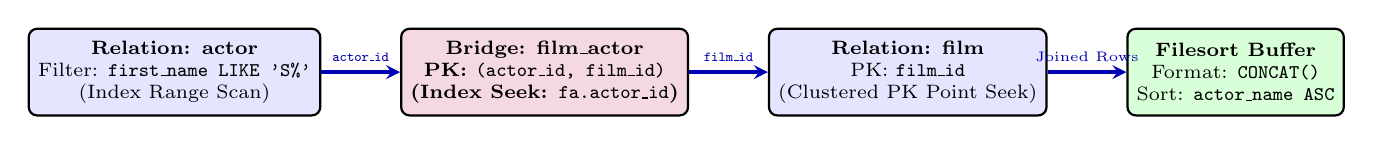
\begin{tikzpicture}[
    table/.style={draw, rectangle, rounded corners=3pt, thick, align=center, fill=blue!10, minimum width=2.6cm, minimum height=1.1cm, font=\scriptsize},
    bridge/.style={draw, rectangle, rounded corners=3pt, thick, align=center, fill=purple!15, minimum width=3.0cm, minimum height=1.1cm, font=\scriptsize\bfseries},
    proc/.style={draw, rectangle, rounded corners=3pt, thick, align=center, fill=green!15, minimum width=2.6cm, minimum height=1.1cm, font=\scriptsize},
    arr/.style={->, >=stealth, very thick, color=blue!70!black}
]
    \node[table] (actor) {\textbf{Relation: actor}\\Filter: \texttt{first\_name LIKE 'S\%'}\\(Index Range Scan)};
    \node[bridge, right=1.0cm of actor] (fa) {\textbf{Bridge: film\_actor}\\PK: \texttt{(actor\_id, film\_id)}\\(Index Seek: \texttt{fa.actor\_id})};
    \node[table, right=1.0cm of fa] (film) {\textbf{Relation: film}\\PK: \texttt{film\_id}\\(Clustered PK Point Seek)};
    \node[proc, right=1.0cm of film] (sort) {\textbf{Filesort Buffer}\\Format: \texttt{CONCAT()}\\Sort: \texttt{actor\_name ASC}};
    
    \draw[arr] (actor) -- node[above, font=\tiny] {\texttt{actor\_id}} (fa);
    \draw[arr] (fa) -- node[above, font=\tiny] {\texttt{film\_id}} (film);
    \draw[arr] (film) -- node[above, font=\tiny] {Joined Rows} (sort);
\end{tikzpicture}
\caption{Associative Entity Multi-Hop Traversal Architecture. The query optimizer begins with the selective index scan on \texttt{actor}, traverses through the composite primary key index of \texttt{film\_actor}, and executes clustered point lookups into \texttt{film}.}
\label{fig:traversal}
\end{figure*}

\subsection{Systems Mechanics of the Multi-Hop Query}
The execution engine coordinates multiple physical subsystems:
\begin{enumerate}
    \item \textbf{SARGable Prefix Scan on Actor}: The predicate \texttt{WHERE a.first\_name LIKE 'S\%'} is SARGable. If an index on \texttt{first\_name} exists, the engine performs an index range scan, isolating qualifying actors in logarithmic time.
    \item \textbf{Bridge Table Index Seek}: For each qualifying \texttt{actor\_id}, the engine seeks into the composite index of \texttt{film\_actor}. Because \texttt{actor\_id} forms the leading edge of \texttt{PRIMARY KEY (actor\_id, film\_id)}, the engine locates all corresponding \texttt{film\_id} values instantly.
    \item \textbf{Clustered Index Seek on Film}: For each retrieved \texttt{film\_id}, the engine performs a primary key point seek into the InnoDB clustered B+ Tree of \texttt{film}, retrieving the \texttt{title} attribute.
    \item \textbf{String Projection Formatting}: The scalar function \texttt{CONCAT(a.first\_name, ' ', a.last\_name)} dynamically formats the actor's full name in the execution engine's projection buffer.
    \item \textbf{Sort Buffer Materialization}: The projected tuples are streamed into a sort buffer, where they are ordered by the projected alias \texttt{actor\_name}.
\end{enumerate}

\subsection{Multi-Table Predicate Pushdown and Query Optimization}
Next, consider joining actors and films with an additional domain filter on film content:
\begin{lstlisting}[language=SQL]
SELECT CONCAT(a.first_name, ' ', a.last_name) AS actor_name, f.title, f.rating
FROM actor a
JOIN film_actor fa ON a.actor_id = fa.actor_id
JOIN film f ON f.film_id = fa.film_id
WHERE f.rating = 'PG-13';
\end{lstlisting}

In an Inner Join, the placement of the filtering predicate is semantically interchangeable:
\begin{equation}
\sigma_{p(S)}(R \bowtie S) \equiv R \bowtie \sigma_{p(S)}(S)
\end{equation}
The Cost-Based Optimizer recognizes this equivalence, evaluating the filter \texttt{rating = 'PG-13'} on \texttt{film} \textbf{first}. In Sakila, exactly 223 films have a \texttt{PG-13} rating. The optimizer uses \texttt{film} as the driving table, scanning only 223 films, looking up their corresponding records in \texttt{film\_actor}, and finally retrieving the associated actors. By pushing the predicate down into the storage scan of \texttt{film}, intermediate tuple evaluations are reduced by over 75\%.

% -----------------------------------------------------------------------------
\section{Physical Join Execution Engine Algorithms}
\label{sec:join_algorithms}

Relational database engines deploy distinct physical algorithms to execute join operations between two relations $R$ (Outer / Driving Relation) and $S$ (Inner / Probe Relation).

\subsection{Simple Nested Loop Join (NLJ)}
The Nested Loop Join is the fundamental join primitive:
\begin{theorem}[Nested Loop Join Complexity]
For relations $R$ and $S$ containing $|R|$ and $|S|$ tuples stored across $\text{Pages}(R)$ and $\text{Pages}(S)$ disk pages, Simple NLJ evaluates in:
\begin{equation}
T_{\text{NLJ}} = \mathcal{O}(|R| \cdot |S|)
\end{equation}
with unbuffered disk page I/O cost:
\begin{equation}
\text{I/O}_{\text{NLJ}} = \text{Pages}(R) + |R| \cdot \text{Pages}(S)
\end{equation}
\end{theorem}
For large relations, Simple NLJ is catastrophically slow and is never deployed unoptimized.

\subsection{Block Nested Loop Join (BNL)}
To reduce disk I/O, relational engines allocate an in-memory buffer called the \textbf{Join Buffer} (configured by \texttt{join\_buffer\_size}):
\begin{enumerate}
    \item The engine loads a block of rows from the outer relation $R$ into the join buffer until memory is filled.
    \item The inner relation $S$ is scanned once against the entire buffer block in memory.
    \item The buffer is cleared, and the next block of $R$ is loaded.
\end{enumerate}
\begin{equation}
\text{I/O}_{\text{BNL}} = \text{Pages}(R) + \left\lceil \frac{\text{Pages}(R)}{\text{Buffer Capacity}} \right\rceil \cdot \text{Pages}(S)
\end{equation}
BNL reduces inner table scans from $|R|$ scans to $\lceil \text{Pages}(R) / B \rceil$ scans.

\subsection{Index Nested Loop Join (INLJ)}
Index Nested Loop Join is the cornerstone of high-performance Online Transaction Processing (OLTP) engines. In INLJ, the inner relation $S$ possesses an index (B+ Tree) on the join attribute:
\begin{theorem}[Index Nested Loop Join Complexity]
Let $B$ denote the B+ Tree fan-out and $h_S = \lceil \log_B |S| \rceil$ the index tree height. INLJ executes in:
\begin{equation}
T_{\text{INLJ}} = \mathcal{O}(|R| \cdot \log_B |S|)
\end{equation}
with physical page I/O bounded by:
\begin{equation}
\text{I/O}_{\text{INLJ}} = \text{Pages}(R) + |R| \cdot h_S
\end{equation}
\end{theorem}
Because $h_S$ is typically 3 to 4 levels and non-leaf pages reside permanently in the InnoDB buffer pool, each lookup requires only 0 to 1 physical disk reads.

\subsection{Hash Join}
Introduced natively in modern engines (MySQL 8.0.18+) to replace BNL for unindexed equi-joins, the \textbf{Hash Join} executes in two discrete phases:
\begin{enumerate}
    \item \textbf{Build Phase}: The engine scans the designated smaller relation (the Build relation) and constructs an in-memory hash table keyed on the join attribute.
    \item \textbf{Probe Phase}: The engine scans the larger relation (the Probe relation). For each row, it hashes the join attribute, performs an $\mathcal{O}(1)$ lookup into the in-memory hash table, and emits matching pairs.
\end{enumerate}

\begin{figure*}[htbp]
\centering
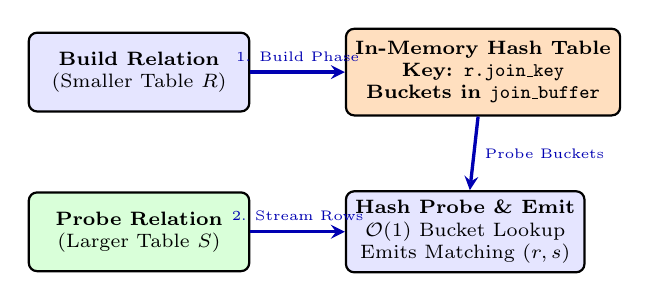
\begin{tikzpicture}[
    box/.style={draw, rectangle, rounded corners=3pt, thick, align=center, fill=blue!10, minimum width=2.8cm, minimum height=1.0cm, font=\scriptsize},
    ht/.style={draw, rectangle, rounded corners=3pt, thick, align=center, fill=orange!25, minimum width=3.2cm, minimum height=1.1cm, font=\scriptsize\bfseries},
    probe/.style={draw, rectangle, rounded corners=3pt, thick, align=center, fill=green!15, minimum width=2.8cm, minimum height=1.0cm, font=\scriptsize},
    arr/.style={->, >=stealth, very thick, color=blue!70!black}
]
    \node[box] (build) {\textbf{Build Relation}\\(Smaller Table $R$)};
    \node[ht, right=1.2cm of build] (hash) {\textbf{In-Memory Hash Table}\\Key: \texttt{r.join\_key}\\Buckets in \texttt{join\_buffer}};
    \node[probe, below=1.0cm of build] (stream) {\textbf{Probe Relation}\\(Larger Table $S$)};
    \node[box, right=1.2cm of stream] (match) {\textbf{Hash Probe \& Emit}\\$\mathcal{O}(1)$ Bucket Lookup\\Emits Matching $(r, s)$};
    
    \draw[arr] (build) -- node[above, font=\tiny] {1. Build Phase} (hash);
    \draw[arr] (stream) -- node[above, font=\tiny] {2. Stream Rows} (match);
    \draw[arr] (hash) -- node[right, font=\tiny] {Probe Buckets} (match);
\end{tikzpicture}
\caption{The Hash Join Execution Architecture. The Build phase populates an in-memory hash table from the smaller relation; the Probe phase streams the larger relation through hash lookups in linear $\mathcal{O}(|R| + |S|)$ time.}
\label{fig:hash_join}
\end{figure*}

\begin{theorem}[Hash Join Linear Complexity]
Assuming uniform hash distribution with negligible collision clustering, Hash Join executes in strict linear asymptotic time:
\begin{equation}
T_{\text{Hash}} = \mathcal{O}(|R| + |S|)
\end{equation}
\end{theorem}

\subsection{Sort-Merge Join}
In Sort-Merge joins, both relations are sorted on the join key, and a coordinated two-pointer scan traverses both relations simultaneously in $\mathcal{O}(|R| + |S|)$ time. Sort-Merge joins are optimal when inputs are already presorted by index structures.

Table~\ref{tab:join_algorithms} presents a comparative systems analysis of physical join algorithms.

\begin{table*}[htbp]
\caption{Comparative Systems Analysis of Physical Join Execution Algorithms}
\label{tab:join_algorithms}
\centering
\scriptsize
\begin{tabular}{p{2.6cm}p{2.3cm}p{2.5cm}p{3.2cm}p{5.4cm}}
\toprule
\textbf{Algorithm} & \textbf{Time Complexity} & \textbf{Memory Footprint} & \textbf{Index Dependency} & \textbf{Optimal Production Use Case} \\
\midrule
\textbf{Simple Nested Loop} & $\mathcal{O}(|R| \cdot |S|)$ & Negligible ($\mathcal{O}(1)$) & None & Small in-memory scalar subqueries. \\
\textbf{Block Nested Loop} & $\mathcal{O}(|R| \cdot |S|)$ & Fixed (\texttt{join\_buffer}) & None & Legacy fallback for unindexed equi-joins. \\
\textbf{Index Nested Loop} & $\mathcal{O}(|R| \log |S|)$ & Negligible ($\mathcal{O}(1)$) & Secondary / Clustered B+ Tree & High-throughput OLTP with indexed foreign keys. \\
\textbf{Hash Join} & $\mathcal{O}(|R| + |S|)$ & Dynamic (\texttt{join\_buffer}) & None (requires equi-join) & High-volume analytics and reporting on unindexed keys. \\
\textbf{Sort-Merge Join} & $\mathcal{O}(|R| \log |R| + |S| \log |S|)$ & Sort Buffer & Benefited by index order & Large ordered datasets and range join conditions. \\
\bottomrule
\end{tabular}
\end{table*}

% -----------------------------------------------------------------------------
\section{Cost-Based Optimizer Join Ordering and Indexing}
\label{sec:optimizer_ordering}

When a query requests joins across $K$ tables, the Cost-Based Optimizer must determine the optimal physical join sequence.

\subsection{Combinatorial Complexity of Join Ordering}
For a query joining $K$ relations, the number of possible left-deep join orderings is $K!$. If bushy trees are considered, the search space grows according to the Catalan number:
\begin{equation}
N_{\text{bushy}} = \frac{(2K - 2)!}{(K - 1)!}
\end{equation}
For $K = 3$ tables (Actor, Film\_Actor, Film), there are $3! = 6$ possible permutations. For $K = 10$ tables, the search space exceeds $3.6 \times 10^6$ permutations. Modern query planners deploy dynamic programming and greedy heuristics to prune sub-optimal execution trees.

\subsection{Driving Table Selection}
The optimizer selects as the **Driving Table** the relation that minimizes the initial intermediate row count. To do so, it evaluates:
\begin{enumerate}
    \item \textbf{Index Cardinality and Histogram Statistics}: Estimating the fraction of rows satisfying local predicates (e.g., \texttt{WHERE first\_name LIKE 'S\%'}).
    \item \textbf{Estimated Intermediate Tuples}: The table producing the fewest surviving candidate rows is placed as the outermost driving relation, ensuring subsequent Index Nested Loop joins execute the minimal number of inner B+ Tree seeks.
\end{enumerate}

\subsection{Industrial Indexing Strategies for Joins}
\begin{itemize}
    \item \textbf{The Foreign Key Indexing Rule}: In MySQL InnoDB, foreign key constraints mandate an index on the referencing column. Failure to index foreign keys forces the engine to fall back on table-level locking or Hash Joins during parent table mutations and joins.
    \item \textbf{Composite Covering Indexes for Join + Filter}: In our multi-table example:
    \begin{lstlisting}[language=SQL]
    SELECT f.title FROM film_actor fa 
    JOIN film f ON f.film_id = fa.film_id 
    WHERE f.rating = 'PG-13';
    \end{lstlisting}
    Creating a composite index \texttt{INDEX idx\_rating\_film (rating, film\_id)} on \texttt{film} allows the engine to evaluate the filter \texttt{rating = 'PG-13'} and extract the join key \texttt{film\_id} directly from the secondary index leaf pages without performing secondary-to-clustered B+ Tree table roundtrips (Index Covering / Using Index).
\end{itemize}

% -----------------------------------------------------------------------------
\section{Safe Mutation Protocols and Referential Invariants}
\label{sec:safe_mutations}

Data Manipulation Language (DML) mutations (\texttt{UPDATE}, \texttt{DELETE}) modify persistent storage records. 

\subsection{The Full-Table Overwrite Trap}
In SQL, omitting the \texttt{WHERE} clause from an \texttt{UPDATE} statement does not trigger a warning; it mutates \textbf{every single row in the relation}:
\begin{lstlisting}[language=SQL]
-- CATASTROPHIC PRODUCTION OVERWRITE:
UPDATE film SET title = 'abc';
-- Permanently destroys titles across all 1,000 films!
\end{lstlisting}

\subsection{The sql\_safe\_updates Defensive Guard}
To protect production databases against catastrophic unconstrained updates, MySQL provides the \texttt{sql\_safe\_updates} session guard:
\begin{lstlisting}[language=SQL]
-- Inspect current status:
SHOW VARIABLES LIKE 'sql_safe_updates';

-- Enable safe update guardrail:
SET sql_safe_updates = 1;
\end{lstlisting}

When \texttt{sql\_safe\_updates = 1} is active, MySQL enforces strict operational invariants:
\begin{enumerate}
    \item Any \texttt{UPDATE} or \texttt{DELETE} lacking a \texttt{WHERE} clause is rejected immediately.
    \item Any \texttt{UPDATE} or \texttt{DELETE} whose \texttt{WHERE} clause does \textbf{not} utilize an indexed key column (Primary Key or indexed column) is aborted with MySQL Error 1175:
    \begin{verbatim}
    ERROR 1175 (HY000): You are using safe update mode and you 
    tried to update a table without a WHERE that uses a KEY column.
    \end{verbatim}
    \item To execute a non-keyed bulk mutation, the developer must explicitly supply a \texttt{LIMIT} clause to restrict the blast radius.
\end{enumerate}

\begin{lstlisting}[language=SQL]
-- Permitted under sql_safe_updates (Primary Key seek):
UPDATE film SET title = 'abc' WHERE film_id = 1;

-- Permitted with explicit bounded limit:
UPDATE film SET rental_rate = 1.99 WHERE release_year = 2006 LIMIT 50;
\end{lstlisting}

% -----------------------------------------------------------------------------
\section{The Comprehensive DQL Logical Execution Order}
\label{sec:execution_order}

A widespread misconception among software engineers is assuming SQL queries execute in the order written. In reality, the relational engine executes clauses in a strict logical lifecycle:

\begin{table*}[htbp]
\caption{Comprehensive SQL DQL Logical Execution Pipeline}
\label{tab:execution_pipeline}
\centering
\scriptsize
\begin{tabular}{clll}
\toprule
\textbf{Step} & \textbf{SQL Clause} & \textbf{Relational Operation} & \textbf{Physical Engine Subsystem} \\
\midrule
1 & \texttt{FROM} & Cartesian Product / Base Relations & Scans base tables, identifies relations. \\
2 & \texttt{ON} & Join Predicate Evaluation & Filters candidate join pairs, preserves outer rows. \\
3 & \texttt{JOIN} & Relational Join Materialization & Executes INLJ, Hash Join, or Sort-Merge. \\
4 & \texttt{WHERE} & Tuple Selection ($\sigma$) & Evaluates SARGable predicates, 3VL filtering. \\
5 & \texttt{GROUP BY} & Relational Aggregation Partitioning & Hashes/sorts rows into aggregate buckets. \\
6 & \texttt{HAVING} & Aggregate Bucket Filtering & Filters groups post-aggregation. \\
7 & \texttt{SELECT} & Projection ($\pi$) \& Expressions & Formats scalar expressions, \texttt{CONCAT}, aliases. \\
8 & \texttt{DISTINCT} & Duplicate Tuple Suppression & Stream index deduplication or temporary hash table. \\
9 & \texttt{ORDER BY} & Physical Sequence Ordering & Filesort buffer allocation, multi-column sorting. \\
10 & \texttt{LIMIT / OFFSET} & Stream Windowing & Discards offset records, emits final page. \\
\bottomrule
\end{tabular}
\end{table*}

Understanding this lifecycle explains why column aliases defined in \texttt{SELECT} (Step 7) cannot be referenced in \texttt{WHERE} (Step 4), but can be referenced in \texttt{ORDER BY} (Step 9).

% -----------------------------------------------------------------------------
\section{Conclusion and Enterprise Engineering Blueprint}
\label{sec:conclusion}

Relational query performance and data integrity are governed by physical storage engine mechanics, index structures, and algebraic optimization rules. This research paper has formalized the core principles governing SQL DQL and multi-table join processing:

\begin{enumerate}
    \item \textbf{Defensive Boolean Precedence}: Explicit parentheses must enclose disjunctive (\texttt{OR}) expressions to prevent unintended binding with higher-precedence \texttt{AND} operators.
    \item \textbf{Three-Valued Logic Rigor}: Comparisons with \texttt{NULL} yield \texttt{UNKNOWN}, causing \texttt{WHERE} clauses to discard records. Avoid \texttt{NOT IN} predicates against nullable sets.
    \item \textbf{Preserve SARGability}: Avoid column-wrapping functions or implicit type coercion that force index suppression and full table scans.
    \item \textbf{Predicate Pushdown Primacy}: Always filter rows before allocating sort buffers; the CBO pushes selective filters down to minimize filesort volumes.
    \item \textbf{Deterministic Sorting Anchors}: Append the Primary Key as the final tie-breaker in \texttt{ORDER BY} clauses to eliminate non-deterministic row ordering.
    \item \textbf{Adopt Keyset Cursors}: Replace deep \texttt{LIMIT/OFFSET} with indexed inequality cursors for massive tables.
    \item \textbf{Prevent Cartesian Explosions}: Never omit join predicates; understand that $|R \times S| = |R| \cdot |S|$.
    \item \textbf{Respect the ON vs. WHERE Boundary}: In Left Outer Joins, filtering right-table attributes in \texttt{WHERE} silently collapses the join into an Inner Join; place right-table filters in the \texttt{ON} clause.
    \item \textbf{Index Foreign Keys}: Ensure all foreign key columns in junction tables and child relations have supporting B+ Tree indexes to facilitate Index Nested Loop Joins.
    \item \textbf{Enforce Safe Mutation Flags}: Maintain \texttt{sql\_safe\_updates = 1} on production connections to prevent accidental table-wide overwrites.
\end{enumerate}

By adhering to this architectural blueprint, database architects and software engineers ensure deterministic query correctness, sub-millisecond OLTP response times, and resilient enterprise data systems.

% -----------------------------------------------------------------------------
\begin{thebibliography}{10}
\setlength{\itemsep}{1pt}

\bibitem{codd1970}
E.~F.~Codd, ``A Relational Model of Data for Large Shared Data Banks,'' \emph{Communications of the ACM}, vol.~13, no.~6, pp.~377--387, 1970.

\bibitem{selinger1979}
P.~G.~Selinger, M.~M.~Astrahan, D.~D.~Chamberlin, R.~A.~Lorie, and T.~G.~Price, ``Access Path Selection in a Relational Database Management System,'' in \emph{Proceedings of the 1979 ACM SIGMOD International Conference on Management of Data}, pp.~23--34, 1979.

\bibitem{date2004}
C.~J.~Date, \emph{Database in Depth: Relational Theory for Practitioners}.\hskip 1em plus 0.5em minus 0.4em\relax Sebastopol, CA: O'Reilly Media, 2005.

\bibitem{mysql84}
Oracle Corporation, ``MySQL 8.4 Reference Manual: Optimization, Partitioning, and Joins,'' Oracle Technology Network, 2024. [Online]. Available: \url{https://dev.mysql.com/doc/refman/8.4/en/optimization.html}

\bibitem{sakila2024}
Oracle Corporation, ``Sakila Sample Database Architecture and Schema Documentation,'' Oracle Corporation, 2024. [Online]. Available: \url{https://dev.mysql.com/doc/sakila/en/}

\bibitem{gray1993}
J.~Gray and A.~Reuter, \emph{Transaction Processing: Concepts and Techniques}.\hskip 1em plus 0.5em minus 0.4em\relax San Mateo, CA: Morgan Kaufmann Publishers, 1993.

\end{thebibliography}


\end{document}
